\documentclass{article}

\usepackage[english]{babel}
\usepackage{float}

\usepackage{graphicx}
\usepackage[colorlinks=true, allcolors=blue]{hyperref}

\usepackage[letterpaper,top=2cm,bottom=2cm]{geometry}

\usepackage{listings}
\usepackage{xcolor}

\definecolor{codegreen}{rgb}{0,0.6,0}
\definecolor{codegray}{rgb}{0.5,0.5,0.5}
\definecolor{codepurple}{rgb}{0.58,0,0.82}
\definecolor{backcolour}{rgb}{0.95,0.95,0.92}

\lstdefinestyle{mystyle}{
    backgroundcolor=\color{backcolour},   
    commentstyle=\color{codegreen},
    keywordstyle=\color{magenta},
    numberstyle=\tiny\color{codegray},
    stringstyle=\color{codepurple},
    basicstyle=\ttfamily\footnotesize,
    breakatwhitespace=false,         
    breaklines=true,                 
    captionpos=b,                    
    keepspaces=true,                 
    numbers=left,                    
    numbersep=5pt,                  
    showspaces=false,                
    showstringspaces=false,
    showtabs=false,                  
    tabsize=2
}

\lstset{style=mystyle}

\date{March 12, 2025}
\title{Assignment 1}
\author{Terrence Jackson}

\begin{document}
\maketitle

\section{Problem 1}


\begin{enumerate}
    \item The linear regression model $ h(\theta) = \theta_0 + \theta_1x_1 $ 

    \item This is the final regression model plot: 

    \begin{figure}[h]
        \centering
        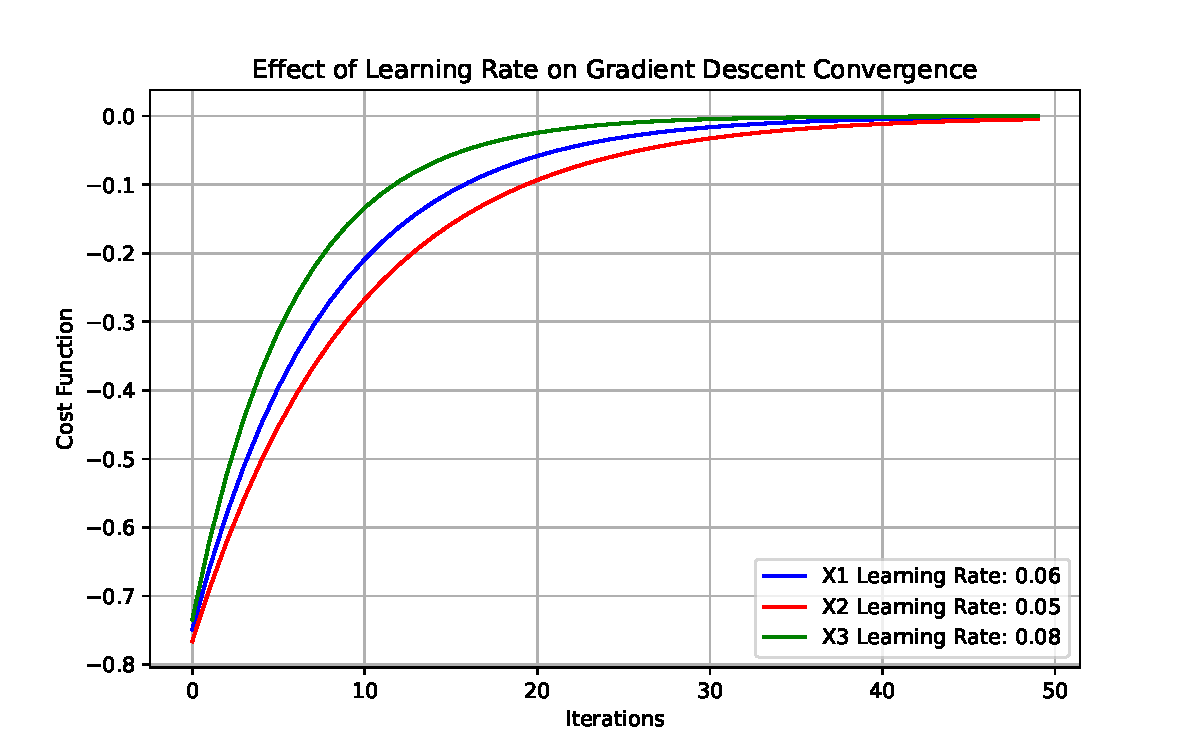
\includegraphics[width=0.9 \linewidth]{ECGR5105/regressionModel.pdf}
        \caption{\label{fig:graph} Linear Regression Model }
    \end{figure}

    \item Over 30 iterations with a learn rate of .08 X3 has the lowest cost.
    \item Learn rate - It seems like the learn rate makes a big difference in the cost conclusions. 


\end{enumerate}

 
\section{Problem 2}

\begin{enumerate}
    \item The best linear regression model $ h(\theta) = \theta_0 + \theta_1x_1 $ 

    \item Loss over interation plot: 

    \begin{figure}[h]
        \centering
        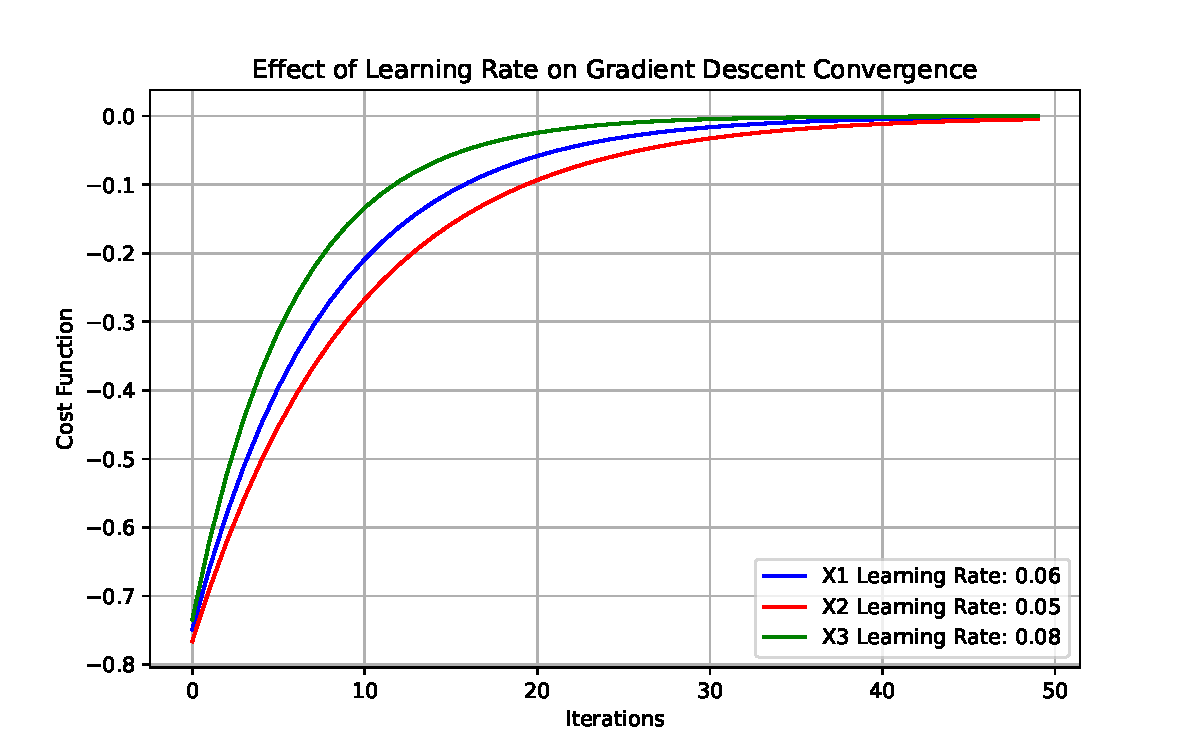
\includegraphics[width=0.9 \linewidth]{ECGR5105/regressionModel.pdf}
        \caption{\label{fig:graph} Linear Regression Model }
    \end{figure}

    \item Based on your training observations, describe the impact of the different learning rates on the final loss and number of training iterations.
    \item Predict the value of y for new (x1, x2, x3) values: (1, 1, 1), (2, 0, 4), and (3, 2, 1)


\end{enumerate}


\section{Code}

\lstinputlisting[language=bash]{Asst1.py}

\section{Additional Info}

Terrence Jackson

ID: tjack121

Assignment 1 

GitHub URL: 
\url{https://github.com/tjackson0678/TestSite/tree/main/python/ECGR5105}

\end{document}